\frame{\frametitle{Model Image}
\begin{figure}
	\centering
   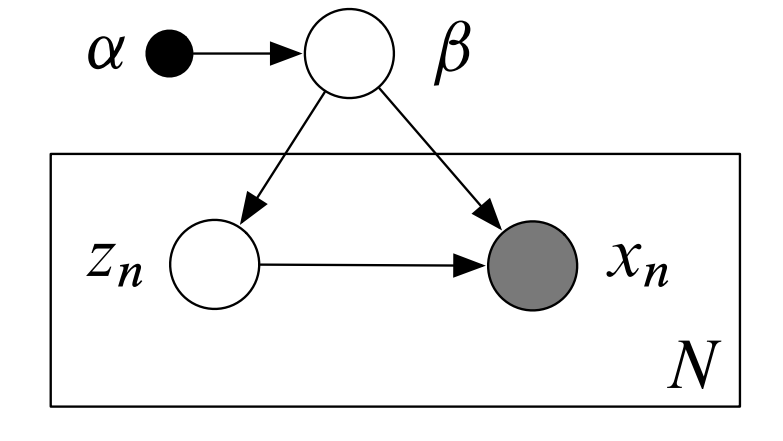
\includegraphics[scale=.25]{figs/fig2-model}
\end{figure}

\begin{table}
\centering
\begin{tabular}{cccc}
\textbf{Variable} & \textbf{Known} & \textbf{Jason's Term} & \textbf{Examples}\\
$x_n$ & observed & input & words (HMM POS, LDA)\\ \hline
\multirow{2}{*}{$z_n$} & \multirow{2}{*}{latent} & output & POS tags, topic assignments\\ 
 &  & nuissance & POS transition probabilities\\  \hline
$\beta$ & latent & nuissance & topic priors\\ \hline
$\alpha$ & either & nuissance & hyperparameter \\
\end{tabular}
\end{table}
%give gloss of variables: relate them to the input/output/nuissance ones Jason defines
}